% Gemini theme
% https://github.com/anishathalye/gemini
%
% We try to keep this Overleaf template in sync with the canonical source on
% GitHub, but it's recommended that you obtain the template directly from
% GitHub to ensure that you are using the latest version.

\documentclass[final]{beamer}

% ====================
% Packages
% ====================
\usepackage[style=numeric,backend=biber]{biblatex}
\addbibresource{self-ref-2026.bib}
%\addbibresource{poster.bib}
\usepackage[english]{babel}
\usepackage[strict]{csquotes}% Recommended
\usepackage[T1]{fontenc}
\usepackage{lmodern}
%\usepackage[size=a0,width=120,height=72,scale=1.0]{beamerposter}
\usepackage[size=a0,orientation=landscape,scale=0.75]{beamerposter}
\usetheme{gemini}
\usecolortheme{gemini}
%\usepackage{graphicx}
\usepackage{braket} %Dirac notation
\usepackage{booktabs}
%\usepackage{tikz}
%\usepackage{pgfplots}
\usepackage{amsfonts} 
%\pgfplotsset{compat=1.14}
\setlength{\parskip}{0.5em}

% ====================
% Lengths
% ====================

% If you have N columns, choose \sepwidth and \colwidth such that
% (N+1)*\sepwidth + N*\colwidth = \paperwidth
\newlength{\sepwidth}
\newlength{\colwidth}
\setlength{\sepwidth}{0.025\paperwidth}
\setlength{\colwidth}{0.3\paperwidth}

\newcommand{\separatorcolumn}{\begin{column}{\sepwidth}\end{column}}

% ====================
% Title
% ====================

\title{It from Bit via G\"odel}

\author{John D. Small}

% ====================
% Footer (optional)
% ====================

\footercontent{
   \hfill
  Quantum Information and Probability: from Foundations to Engineering, V\"axj\"o, Sweden, 2026 \hfill
  \href{mailto:john.small06@alumni.imperial.ac.uk}{john.small06@alumni.imperial.ac.uk}
  }
% (can be left out to remove footer)

% ====================
% Logo (optional)
% ====================

% use this to include logos on the left and/or right side of the header:
% \logoright{\includegraphics[height=7cm]{logo1.pdf}}
% \logoleft{\includegraphics[height=7cm]{logo2.pdf}}

% ====================
% Body
% ====================

\begin{document}

\begin{frame}[t]
\begin{columns}[t]
\separatorcolumn

\begin{column}{\colwidth}

  \begin{block}{Self-reference}

    Quantum states have the curious property that they are precisely the states required to represent the classically inadmissible states which occur in self-referential logic, such as the Liar Paradox. The fact that a superposition of $\ket{TRUE}$ and $\ket{FALSE}$ is a perfectly reasonable quantum state and also a fixed point of the Liar Paradox is a pretty big clue. Therefore all interpretations need to find ways to accommodate this property, and all constructionist models need to sneak self-reference in, but disguised as something else, retro-causality, epistemological limitations on knowledge, reversible continuity, negative probability, and so on. See \autocite{svozil_k_2018} and references therein for a full review. In addition it has been suggested that self-reference is the key principle which distinguishes quantum from classical mechanics, \autocite{wheeler_j_1974, szangolies_j_2018, Realpe-Gomez2017} and it has been proved that non-computability plays a key role in quantum mechanics \autocite{calude_2006, bendersky_non_computable_2016}.
    \begin{figure}
        \centering
        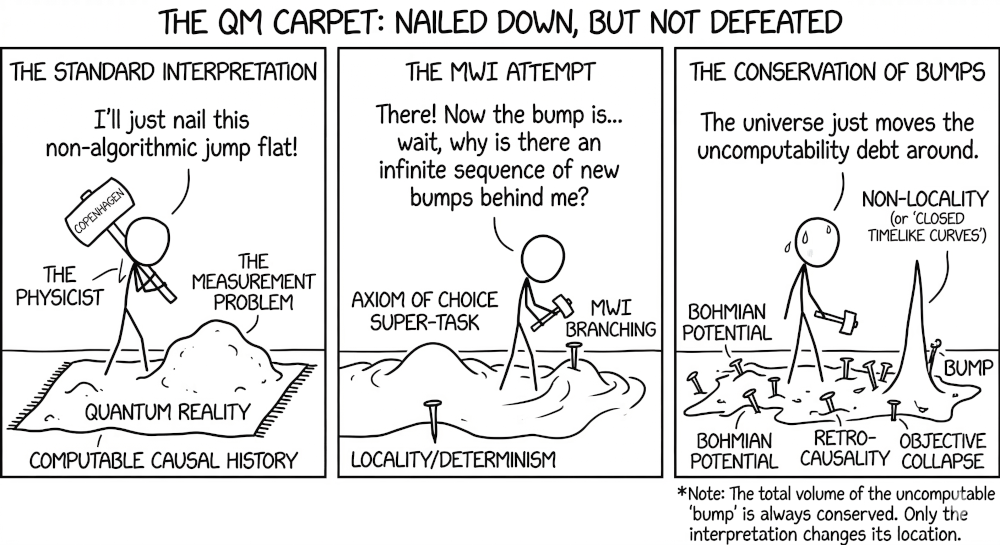
\includegraphics[width=0.95\linewidth]{Gemini_Generated_Image_scaled.png}
        \caption{All interpretations of QM try to nail down non-computability into computability, with a left over bump}
    \end{figure}
    \par
    Rather than hide self-reference behind such terms as \textquote{reversible continuity}, \textquote{retrocausality} or \textquote{epistemic limitations}, \textquote{non-computability} it's better to be completely open about it, state that self-reference is the fundamental postulate that differentiates quantum from classical mechanics and then move on to see if we can do anything useful with the idea.
    \par
    We find that recognising self-reference, non-computability, is fundamental, as suggested by Wheeler \autocite{wheeler_j_1974, wheeler_1988} yet constrained to be viewed as non-self-reference and computable, nailing down the carpet, completely constrains the form of physical law \autocite{small_2006}
  \end{block}
  \begin{block}{Principle Results}
The framework yields three classes of result: structural derivations of Standard Model architecture (gauge group, particle content, spacetime dimensionality), quantitative predictions for masses and couplings, and falsifiable non-observation predictions. We summarise each in turn.


\begin{enumerate}
  \item \textbf{Gauge group.} The Standard Model gauge group $G_{\mathrm{SM}} = SU(3) \times SU(2) \times U(1)/\mathbb{Z}_6$ is the equivariance group of the octonionic Hopf fibration $S^7 \to S^{15} \to S^8$ after selection of the preferred complex direction $\mathbb{C} \subset \mathbb{O}$ forced by the Moufang loop closure.

  \item \textbf{Particle content.} The complete Standard Model particle spectrum is in bijection with the entanglement primitives of three Cayley--Dickson qubits, with exhaustiveness guaranteed by three independent termination theorems: Hurwitz (no division algebras beyond~$\mathbb{O}$) \autocite{hurwitz_1898}, Adams (no Hopf fibrations beyond the octonionic case) \autocite{adams_1960}, and Coecke-Kissinger (compositional completeness of GHZ and W classes) \autocite{Coecke2010TheEntanglement}. (Note that it's an open problem to show that Coecke-Kissinger $\iff$ Adams) 

  \item \textbf{Spacetime dimensionality.} The requirement that state reduction on the Bloch sphere be consistent with Lorentz boosts demands $\mathrm{Spin}(1,d) \cong SL(2,\mathbb{A})$ for a normed division algebra~$\mathbb{A}$. The computability split selects $\mathbb{A} = \mathbb{C}$, giving $SL(2,\mathbb{C}) = \mathrm{Spin}(1,3)$ and thus $d = 3$ spatial dimensions. The six internal dimensions of $SU(3) \times SU(2) \times U(1)$ account for the reduction from $d = 9$ (the octonionic case) to $d = 3$, reproducing the Kaluza--Klein dimensional decomposition $9+1 = (3+1) + 2 + 4$ with a structural explanation.

  \item \textbf{Three generations.} The triality automorphism of $\mathrm{Spin}(8)$, which permutes the three eight-dimensional representations of the octonions, produces exactly three generations of fermions.

  \item \textbf{Chirality.} The non-associativity of $\mathbb{O}$ distinguishes left and right multiplication, breaking parity at the algebraic level.

  \item \textbf{Born rule.} The observer's self-referential ignorance of their own computational state generates a global $U(1)$ phase freedom. The minimum-degree polynomial invariant under this symmetry is $|\psi|^2$, yielding the Born rule without additional postulates.

  \item \textbf{Entanglement monogamy.} The Coffman--Kundu--Wootters inequality follows geometrically from the compactness of the $S^4$ base of the quaternionic Hopf fibration: a ball has a unique centre, and one cannot overshoot it.
\end{enumerate}
  \end{block}
 \begin{block}{Hopf maps. The Key Link}

The idea that entanglement and particle physics share the same algebraic structure is not new. This ideas has been worked on for decades see \autocite{borsten_2009}, but in the context of string/brane theory and therefore impossible to get some actual numbers to compare with experiment. Taking inspiration from Szangolies \autocite{szangolies_2025}, we can map classes of multi-particle entanglement to Standard Model particles and hence transform problems in particle physics into problems in entanglement where easy solutions are possible. The key is that Hopf fibrations (maps) show up both as qubit entanglement classes and in particle physics. 
  \begin{table}[h]
  \centering
  \begin{tabular}{@{}lll@{}}
    \toprule
    \textbf{Entanglement Class} & \textbf{Hopf Map} & \textbf{Particles} \\
    \midrule
    Single qubit (no entanglement) & $S^{1} \to S^{3} \to S^{2}$ & Photon / $U(1)$ electromagnetism \\
    Bell (two-qubit)               & $S^{3} \to S^{7} \to S^{4}$ & $W$, $Z$ / $SU(2)$ weak \\
    W (three-qubit)                & $S^{7} \to S^{15} \to S^{8}$ ($\mathbb{C}$ sector)   & Leptons \\
    GHZ (three-qubit)              & $S^{7} \to S^{15} \to S^{8}$ ($\mathbb{C}^{3}$ sector) & Quarks / $SU(3)$ colour (confined) \\
    \bottomrule
  \end{tabular}
  \caption{Entanglement classes, Hopf fibrations, and the corresponding Standard Model sectors. The three-qubit rows share the octonionic Hopf bundle and split under the computability decomposition $\mathbb{O} \cong \mathbb{C} \oplus \mathbb{C}^{3}$.}
  \label{tab:entanglement-hopf-particles} 
\end{table}
The Higgs is not an entanglement class. It is the Hopf bundle's nontriviality itself, promoted to a dynamical field following \autocite{szangolies_2025, finkelstein_1962, finkelstein_1963}
\end{block}
\end{column}

\separatorcolumn

\begin{column}{\colwidth}

\begin{block}{The non-computable bump shows up as particle mass}
Nailing down non-computabilty in a computable framework leaves a bump in the carpet. This \textquote{logical debt} or \textquote{latent computability} can be interpreted as mass. Using this idea we calculate mass of each charged fermion as given by the generalised Koide formula.
\begin{equation}
  \label{eq:koide}
  \sqrt{m_k} \;=\; M\!\left(1 + \alpha\cos\!\left(\delta + \frac{2\pi k}{3}\right)\right), \qquad k = 0, 1, 2\,,
\end{equation}
where $k$ labels the three generations within each charge sector. The two dimensionless parameters $\alpha$ and $\delta$ are determined by quantum numbers as follows.

\textbf{Koide angle.} The misalignment between the triality-symmetric direction on $\mathbb{O}P^1$ and the preferred complex direction gives
\begin{equation}
  \label{eq:delta}
  \delta_{\mathrm{sector}} \;=\; \frac{\delta_0}{n}\,, \qquad \delta_0 = \frac{\dim_{\mathbb{R}}(\mathbb{C})}{\dim_{\mathbb{R}}(\mathbb{O}P^1)} = \frac{2}{9}\,,
\end{equation}
where $n$ counts the number of active internal fibre directions:
\begin{equation}
  n \;=\; 1 + \bigl(T_3 + \tfrac{1}{2}\bigr) + \mathbf{1}_{\mathrm{colour\,triplet}}\,.
\end{equation}

\textbf{Amplitude parameter.} The ratio of rotation to identity components in the SU(2) holonomy of the self-referential loop gives
\begin{equation}
  \label{eq:alpha}
  \alpha^2 \;=\; 2 + 2\,|Q|^{3/2}\,\mathbf{1}_{\mathrm{colour\,triplet}}\,,
\end{equation}
where $|Q|$ is the magnitude of the electric charge. For charged leptons, $\alpha = \sqrt{2}$ corresponds to a quarter-turn ($\pi/2$) holonomy.

\textbf{Dimensional parameter.} Each charge sector has one free dimensional parameter $M$, fitted to the heaviest observed mass ($m_\tau$, $m_b$, $m_t$). All mass \emph{ratios} within a sector are therefore predictions with zero free parameters.

Table~\ref{tab:inputs} summarises the sector-specific inputs. Table~\ref{tab:masses} presents the resulting mass predictions, and Table~\ref{tab:ratios} presents inter-generation mass ratios.

\begin{table}[t]
  \centering
  \caption{Sector-specific parameters. All dimensionless quantities ($\alpha$, $\delta$) are determined by quantum numbers; only the dimensional scale $M$ is fitted (to the heaviest mass in each sector).}
  \label{tab:inputs}
  \begin{tabular}{lccccccc}
    \toprule
    Sector & $|Q|$ & $T_3$ & Colour & $n$ & $\delta$ & $\alpha^2$ & $M$ fitted to \\
    \midrule
    Charged leptons & 1 & $-\tfrac{1}{2}$ & singlet & 1 & $2/9$ & 2 & $m_\tau$ \\
    Down-type quarks & $\tfrac{1}{3}$ & $-\tfrac{1}{2}$ & triplet & 2 & $1/9$ & $2 + 2/3\sqrt{3}$ & $m_b$ \\
    Up-type quarks & $\tfrac{2}{3}$ & $+\tfrac{1}{2}$ & triplet & 3 & $2/27$ & $2 + 2\sqrt{2/3\sqrt{3}}$ & $m_t$ \\
    \bottomrule
  \end{tabular}
\end{table}

\begin{table}[t]
  \centering
  \caption{Charged fermion mass predictions. Eight of nine masses are reproduced to better than 1.1\% from the single dimensionless constant $\delta_0 = 2/9$ and the quantum numbers of each particle. The up quark discrepancy has an identified mechanism (see text). Measured values from the Particle Data Group; light quark masses are $\overline{\mathrm{MS}}$ at $\mu = 2\;\mathrm{GeV}$.}
  \label{tab:masses}
  \begin{tabular}{lrrr}
    \toprule
    Particle & Predicted (MeV) & Measured (MeV) & Deviation \\
    \midrule
    $e$ & 0.5110 & 0.5110 & $-0.01\%$ \\
    $\mu$ & 105.652 & 105.658 & $-0.01\%$ \\
    $\tau$ & 1776.86 & 1776.86 & fitted \\[4pt]
    $d$ & 4.62 & 4.67 & $-1.0\%$ \\
    $s$ & 94.4 & 93.4 & $+1.1\%$ \\
    $b$ & 4180 & 4180 & fitted \\[4pt]
    $u$ & 2.78 & 2.16 & $+28.5\%\;^{(*)}$ \\
    $c$ & 1271.4 & 1270 & $+0.1\%$ \\
    $t$ & 172\,500 & 172\,500 & fitted \\
    \bottomrule
  \end{tabular}
\end{table}

\begin{table}[t]
  \centering
  \caption{Inter-generation mass ratios (zero free parameters). All ratios except $m_c/m_u$ are predicted to better than 2\%. The $m_c/m_u$ discrepancy shares the same origin as the up quark mass anomaly.}
  \label{tab:ratios}
  \begin{tabular}{lrrr}
    \toprule
    Ratio & Predicted & Measured & Deviation \\
    \midrule
    $m_\mu / m_e$ & 206.8 & 206.8 & $0.006\%$ \\
    $m_\tau / m_e$ & 3477.5 & 3477.2 & $0.008\%$ \\[4pt]
    $m_s / m_d$ & 20.4 & 20.0 & $2\%$ \\
    $m_b / m_d$ & 903.9 & 895.1 & $1\%$ \\[4pt]
    $m_t / m_c$ & 135.68 & 135.83 & $0.1\%$ \\
    $m_c / m_u$ & 458 & 588 & $22\%\;^{(*)}$ \\
    \bottomrule
  \end{tabular}
\end{table}

\end{block}
\begin{block}{Quantitative predictions: bosonic sector}

The framework yields the following zero-parameter predictions for bosonic quantities:

\begin{table}[h]
  \centering
  \caption{Bosonic sector predictions. All values are derived from the Hopf fibration geometry with no free parameters. The Weinberg angle and strong coupling are tree-level predictions; measured values include radiative corrections via standard renormalisation group evolution with Standard Model particle content.}
  \label{tab:bosons}
  \begin{tabular}{llll}
    \toprule
    Quantity & Predicted & Measured & Deviation \\
    \midrule
    $\sin^2\!\theta_W$ & $1/4$ (tree level) & 0.2312 (at $M_Z$) & consistent after RGE \\
    $m_H$ & $v/2 = 123.1\;\mathrm{GeV}$ & $125.25\;\mathrm{GeV}$ & $\sim 2\%$ \\
    $y_t$ (top Yukawa) & 1 & 0.991 & $\sim 1\%$ \\
    $\alpha_s(M_Z)$ & $\approx 0.1185$ & 0.1179 & $\sim 0.5\%$ \\
    $\theta_{\mathrm{QCD}}$ & 0 (topological) & $< 10^{-10}$ & consistent \\
    \bottomrule
  \end{tabular}
\end{table}

The Weinberg angle prediction $\sin^2\!\theta_W = 1/4$ arises from the equal-weight projection on the $S^4$ base of the quaternionic Hopf fibration. This is a tree-level (UV) value; running to $M_Z$ via the standard one-loop renormalisation group equations with the known Standard Model particle content yields $\sin^2\!\theta_W(M_Z) \approx 0.231$, in agreement with the measured value.

\textbf{The strong CP angle $\theta_{\mathrm{QCD}} = 0$ is topologically forced}: the GHZ entanglement class characterising quarks has maximal three-tangle ($\tau_3 = 1$) and zero pairwise concurrence, precluding the oriented linking structure that would generate a non-trivial vacuum angle.
\end{block}
\end{column}

\separatorcolumn

\begin{column}{\colwidth}

\begin{block}{Non-observation predictions}

In addition to the quantitative predictions above, the framework makes several structural predictions that take the form of strict non-observations:

\begin{enumerate}
  \item \textbf{No supersymmetric partners.} The division algebra tower terminates at $\mathbb{O}$; no algebraic structure exists to support a boson$\leftrightarrow$fermion symmetry. Confirmed by LHC Run~1 and Run~2 null results.

  \item \textbf{No proton decay.} The gauge group $G_{\mathrm{SM}}$ arises from parallelisable spheres, which do not produce $SU(5)$ or any other simple group containing $G_{\mathrm{SM}}$. Baryon number violation via leptoquark exchange is therefore structurally absent. Consistent with Super-Kamiokande bounds ($\tau_p > 10^{34}$~years).

  \item \textbf{All Flavor Changing Neutral Current top quark decays via neutral bosons are exactly zero at all orders.} Generation labels correspond to triality sectors (octonion associator bracketings); neutral bosons ($Z$, $\gamma$, gluon, Higgs) have no mechanism to change bracketing. This is a structural prohibition, stronger than the SM's GIM cancellation. All ATLAS Run~2 searches are consistent with null results. The HL-LHC programme will probe BSM-enhanced rates of $10^{-5}$--$10^{-4}$; the framework predicts these searches will remain null.

  \item \textbf{Neutrino mass sum $\Sigma m_\nu = 2.6\;\mathrm{meV}$, normal ordering.} Testable by DESI, Euclid, and CMB-S4 within the next decade. An inverted mass ordering would falsify the framework.
\end{enumerate}
\end{block}
\begin{block}{Quantum Circuits}
 Because we can use Hopf maps to go from particle physics to multi-qubit entanglement then we can create quantum circuits to emulate particle interactions. See draft paper at;-
 \begin{figure}
     \centering
     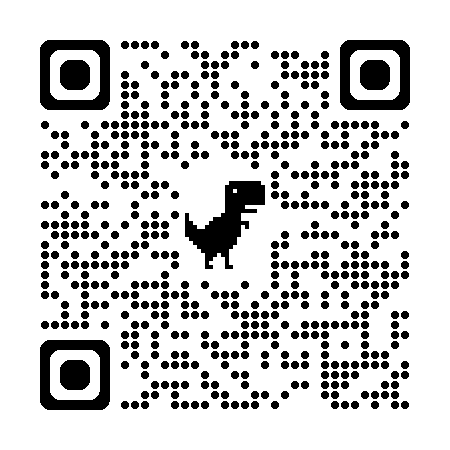
\includegraphics[width=0.5\linewidth]{qrcode_it-from-bit.vidhya.tv.png}
     \caption{Draft paper}
     \label{fig:draft_paper}
 \end{figure}
 This is an evolving project. In the paper I list a lot of open problems to be solved. 
\end{block}

  \begin{block}{References}
    \printbibliography
  \end{block}

\end{column}

\separatorcolumn
\end{columns}
\end{frame}

\end{document}
